\documentclass[12pt,a4paper]{report}
\usepackage[utf8]{inputenc}
\usepackage[bahasa]{babel}
\usepackage{graphicx}
\usepackage{booktabs}
\graphicspath{{figures/}}
\usepackage{geometry}
\usepackage{setspace}
\usepackage{titlesec}
\usepackage{natbib}
\usepackage{hyperref}
\usepackage{caption}
\usepackage{subcaption}
\usepackage{amsmath}
\usepackage{amssymb}
\usepackage{float}

% Geometry setup
\geometry{
    top=3cm,
    bottom=3cm,
    left=4cm,
    right=3cm
}

% Title format
\titleformat{\chapter}[display]
  {\normalfont\bfseries\centering}{\chaptertitlename\ \thechapter}{20pt}{\Large}
\titleformat{\section}
  {\normalfont\bfseries}{\thesection}{1em}{}
\titleformat{\subsection}
  {\normalfont\bfseries}{\thesubsection}{1em}{}

% Spacing
\onehalfspacing

\begin{document}

% Title Page
\begin{titlepage}
    \centering
    \vspace*{1cm}
    
    {\Large \textbf{Pemetaan Tanaman Pertanian Berbasis Citra Multi-Temporal Sentinel-2 dengan Pendekatan Kombinasi Band Spektral dan Model Semantic Segmentation}}
    
    \vspace{1.5cm}
    
    \textbf{TUGAS AKHIR}
    
    \vspace{1.5cm}
    
    Diajukan sebagai salah satu syarat untuk memperoleh gelar Sarjana Sains Data pada\\
    Program Studi Sarjana Sains Data\\
    Fakultas Informatika Universitas Telkom
    
    \vspace{1.5cm}
    
    \textbf{Oleh:}\\
    \textbf{IZZULHAQ MAHARDIKA}\\
    \textbf{1305220010}
    
    \vspace{1.5cm}
    
    \textbf{Pembimbing:}\\
    Dr. Gamma Kosala, S.Si\\
    NIP. 21920013
    
    \vspace{2cm}
    
    \textbf{PROGRAM STUDI SARJANA SAINS DATA}\\
    \textbf{FAKULTAS INFORMATIKA}\\
    \textbf{UNIVERSITAS TELKOM}\\
    \textbf{BANDUNG}\\
    \textbf{2025}
    
\end{titlepage}

\chapter*{Lembar Persetujuan}
\begin{center}
    \textbf{Pemetaan Tanaman Pertanian Berbasis Citra Multi-Temporal Sentinel-2 dengan Pendekatan Kombinasi Band Spektral dan Model Semantic Segmentation}
    \\
    \textit{Crop Mapping Based on Multi-Temporal Sentinel-2 Imagery with Spectral Band Combination and Semantic Segmentation Models}
    \vspace{1cm}
    
    \textbf{Izzulhaq Mahardika}\\
    NIM: 1305220010
    \vspace{1cm}
    
    Tugas Akhir ini diajukan sebagai salah satu syarat untuk memperoleh gelar Sarjana Sains Data pada\\
    Program Studi Sarjana Sains Data\\
    Fakultas Informatika Universitas Telkom\\
    Bandung, 13 Oktober 2025
    \vspace{1cm}
    
    Menyetujui,\\
    Pembimbing
    \vspace{2cm}
    
    \underline{Dr. Gamma Kosala, S.Si}\\
    NIP. 21920013
\end{center}

\chapter*{Abstrak}
Pemetaan tanaman pertanian berperan penting dalam mendukung ketahanan pangan, perencanaan pola tanam, serta pengelolaan sumber daya agrikultur. 
Citra satelit Sentinel-2 dengan resolusi tinggi spasial dan temporal telah banyak dimanfaatkan dalam klasifikasi tutupan lahan, termasuk untuk identifikasi jenis tanaman. 
Penelitian ini mengadopsi pendekatan \textit{semantic segmentation} berbasis \textit{deep learning}, yaitu DeepLabV3+ dan SegFormer, untuk mengklasifikasikan tanaman pertanian berdasarkan citra multi-temporal Sentinel-2 dan label dari \textit{Cropland Data Layer} (CDL) milik USDA. 

Studi literatur menunjukkan bahwa pendekatan multi-temporal dan kombinasi band spektral dapat meningkatkan akurasi klasifikasi karena mampu menangkap dinamika spektral dan fenologi tanaman. 
Area studi terletak di Sacramento Valley, California, yang merupakan salah satu kawasan agrikultur paling produktif di Amerika Serikat. 
Data Sentinel-2 dikumpulkan setiap 15 hari selama periode 2022--2024 dan diproses melalui tahapan \textit{masking} awan, \textit{histogram matching}, \textit{resampling} spasial, normalisasi, dan \textit{patching}. 

Evaluasi dilakukan menggunakan metrik \textit{Overall Accuracy}, \textit{Mean Intersection over Union} (mIoU), dan F1-score, serta dilengkapi analisis kesalahan dan waktu inferensi. 
Penelitian ini juga mengimplementasikan \textit{attention mechanism} pada masing-masing model untuk meningkatkan performa segmentasi. 
Eksperimen dilakukan dalam beberapa skenario yang menguji pengaruh data multi-temporal dan kombinasi spektral terhadap hasil klasifikasi tanaman. 
Hasil dari studi ini diharapkan dapat memberikan kontribusi terhadap pengembangan model segmentasi citra multispektral yang lebih akurat dan adaptif terhadap variasi spasial dan temporal tutupan lahan pertanian.

\vspace{0.5cm}
\textbf{Kata Kunci:} Pemetaan Pertanian, Multi-temporal, Band Spektral, Semantic Segmentation


\tableofcontents
\listoftables
\listoffigures

\chapter{PENDAHULUAN}
\section{Latar Belakang}
Pertumbuhan penduduk dunia dan meningkatnya standar hidup telah mendorong perluasan serta intensifikasi pemanfaatan lahan pertanian secara global untuk memenuhi permintaan pangan dan komoditas yang terus meningkat \citep{potapov2022}. 
Pengembangan peta sebaran tanaman secara akurat dan skala besar menjadi penting untuk memastikan ketahanan pangan dan merencakanan pola tanam di masa depan \citep{gao2023}. 
Informasi spasial mengenai sebaran dan jenis tanaman pertanian sangat dibutuhkan untuk estimasi hasil panen, mengelola irigasi, serta merencanakan distribusi komoditas \citep{yi2020}. 

Satelit penginderaan jauh menyediakan citra resolusi tinggi yang dapat dimanfaatkan untuk pemetaan lahan pertanian secara luas dan otomatis, sebagai alternatif metode survei lapangan konvensional yang memakan waktu dan biaya tinggi \citep{li2023}. 
Satelit Sentinel-2 digunakan untuk pemetaan lahan pertanian karena menyediakan citra dengan resolusi tinggi hingga 10 meter dan resolusi temporal pada 5 hari \citep{phiri2020}. 
Sentinel-2 memiliki hingga 13 band spektral yang dapat dimanfaatkan untuk fitur pada klasifikasi lahan pertanian \citep{yi2020}. 
Penggunaan Cropland Data Layer (CDL) yang disediakan oleh United States Department of Agriculture (USDA) sebagai data label dapat meningkatkan validitas pemetaan tanaman karena menyediakan label hingga tingkat piksel dengan resolusi 30 meter dan cakupan spasial yang luas \citep{maleki2024}. 

Kemajuan dalam bidang \textit{computer vision} (CV) dan \textit{deep learning} menciptakan pergeseran dalam analisis penginderaan jauh menuju metode \textit{semantic segmentation} \citep{luo2024}. 
Berbeda dengan klasifikasi piksel-per-piksel biasa, \textit{semantic segmentation} mengelompokkan piksel dengan kelas tutupan lahan tertentu secara bersamaan \citep{ajibola2024}. 
Algoritma \textit{semantic segmentation} seperti DeepLabV3+ dan SegFormer mulai diadopsi untuk klasifikasi tanaman pertanian \citep{li2023}. 
Model segmentasi lainnya seperti DeepLabV3+ dan SegFormer juga telah diterapkan, salah satunya oleh Li (2023), yang menunjukkan bahwa kedua model tersebut mampu menghasilkan akurasi segmentasi tinggi \citep{li2023, hsu2022, chang2023}. 

Meskipun demikian, beberapa penelitian fokus pada penggunaan citra indeks vegetasi (NDVI, EVI) tanpa mempertimbangkan keunggulan seluruh band spektral \citep{gao2023, thorp2021, seydi2022}. 
Padahal, kombinasi fitur spektral yang dipilih dengan metode \textit{feature selection} dapat meningkatkan pemisahan kelas tanaman \citep{yi2020}. 
Oleh karena itu, diperlukan eksperimen untuk menentukan kombinasi band dan multi-spektral yang optimal, sehingga proses pemetaan tanaman pertanian dapat lebih akurat. 

Pengembangan model \textit{semantic segmentation} berbasis citra satelit memerlukan data label yang akurat hingga level piksel. 
Namun, di Indonesia belum tersedia dataset publik untuk identifikasi jenis tanaman pertanian. 
Untuk mengatasi masalah tersebut, area studi pada penelitian ini difokuskan di kawasan Sacramento Valley, California di Amerika Serikat yang didukung oleh ketersediaan dataset publik Cropland Data Layer (CDL). 

\section{Perumusan Masalah}
Berikut adalah rumusan masalah pada penelitian ini:
\begin{enumerate}
    \item Bagaimana pengaruh dari data multi-temporal pada akurasi pemetaan tanaman?
    \item Bagaimana pengaruh dari kombinasi band spektral yang berbeda pada kinerja model \textit{semantic segmentation}?
    \item Bagaimana kinerja dari beberapa model \textit{semantic segmentation}, DeepLabV3+, dan SegFormer untuk klasifikasi tanaman pertanian?
\end{enumerate}

\section{Tujuan}
Berdasarkan rumusan masalah yang telah disebutkan, tujuan penelitian ini adalah sebagai berikut:
\begin{enumerate}
    \item Mengevaluasi pengaruh dari data multi-temporal pada akurasi pemetaan tanaman.
    \item Menilai pengaruh dari kombinasi band spektral yang berbeda pada kinerja model \textit{semantic segmentation}.
    \item Membandingkan kinerja dari tiga model \textit{semantic segmentation}, DeepLabV3+, dan SegFormer, untuk mengklasifikasikan tanaman pertanian pada citra Sentinel-2.
\end{enumerate}

\section{Batasan Masalah}
Batasan masalah pada penelitian ini adalah sebagai berikut:
\begin{enumerate}
    \item Penelitian ini menggunakan data sekunder dari platform Google Earth Engine (GEE). Dataset terdiri dari atas citra Sentinel-2 sebagai input dan Cropland Data Layer (CDL) sebagai data label, dengan periode pengambilan antara tahun 2022 hingga 2024.
    \item Area studi terletak di kawasan Sacramento Valley, California pada koordinat geografis ($122^{\circ}18'36''$ BB hingga $121^{\circ}20'26''$ BB, $38^{\circ}41'7''$ LU hingga $39^{\circ}49'47''$ LU) dengan total luas area 10.629,25 km$^2$.
\end{enumerate}

\section{Hipotesis}
Berdasarkan temuan studi terdahulu, hipotesis yang diajukan dalam penelitian ini adalah sebagai berikut:
\begin{itemize}
    \item Penggunaan citra multi-temporal dengan kombinasi band spektral menghasilkan dataset yang kaya akan fitur, sehingga akan menghasilkan akurasi pemetaan pertanian yang lebih tinggi dibandingkan penggunaan citra \textit{single-date} atau hanya menggunakan indeks vegetasi.
    \item Model \textit{semantic segmentation} dengan \textit{attention mechanism} dihipotesiskan memiliki performa lebih baik daripada model tanpa attention (\textit{baseline}), karena kemampuannya dalam memfokuskan pada fitur-fitur penting.
\end{itemize}

\section{Rencana Kegiatan}
Untuk mencapai tujuan yang telah ditentukan, penelitian ini akan dilaksanakan melalui tahapan kegiatan sebagai berikut:
\begin{enumerate}
    \item \textbf{Studi Literatur dan Perumusan Metode}\\
    Melakukan kajian pustaka yang relevan terkait pemetaan tanaman pertanian dengan citra satelit, pemanfaatan citra multi-temporal, pemilihan dan kombinasi band spektral Sentinel-2, dan model \textit{semantic segmentation} khususnya DeepLabV3+, dan SegFormer. Berdasarkan kajian ini, dirumuskan kesenjangan penelitian dan kerangka metodologi penelitian.
    
    \item \textbf{Pengumpulan Data}\\
    Mengambil data citra multi-temporal Sentinel-2 untuk area studi di Sacramento Valley dengan spektral band B2, B3, B4, B5, B7, B8, B11, dan B12 dengan interval komposit 15 hari selama setahun penuh pada tahun 2022, 2023, dan 2024. Selain itu, data label diambil dari Cropland Data Layer (CDL) yang disediakan oleh USDA NASS.
    
    \item \textbf{Preprocessing Data}\\
    Melakukan tahap preprocessing citra yang mencakup \textit{cloud masking} dan \textit{shadow masking}, \textit{resampling} dan projection citra Sentinel-2 dan CDL, normalisasi nilai reflectance, pemilihan kombinasi band spektral optimal menggunakan metode \textit{feature selection} berbasis global separation index, dan patching citra dan label menjadi patch berukuran $256\times256$ piksel serta filter labeling untuk patch selain jenis tanaman pertanian.
    
    \item \textbf{Pelatihan Model Semantic Segmentation}\\
    Melatih dan membangingkan performa tiga arsitektur \textit{semantic segmentation}, yaitu DeepLabV3+, dan SegFormer pada dataset yang telah diproses. Beberapa skenario training akan dilakukan untuk membandingkan pengaruh konfigurasi band dan temporal terhadap hasil segmentasi. Untuk setiap model, akan ditambahkan juga \textit{attention mechanism} untuk meningkatkan kemampuan model dalam menyoroti fitur penting.
    
    \item \textbf{Evaluasi dan Analisis Hasil}\\
    Evaluasi utama dilakukan menggunakan metrik evaluasi segmentasi seperti \textit{mean Intersection over Union} (mIoU), \textit{Overall Accuracy} (OA), dan F1-score. Selain evaluasi utama, akan dilakukan evaluasi tambahan berupa \textit{error analysis} dan pengukuran \textit{inference time}. Analisis hasil mencakup perbandingan antar model, pengaruh kombinasi band, serta pengaruh penggunaan data multi-temporal. Visualisasi segmentasi dan distribusi prediksi kelas juga dianalisis untuk mendukung interpretasi hasil kuantitatif.
    
    \item \textbf{Penyusunan Laporan Akhir}\\
    Menyusun laporan akhir tugas akhir yang berisi latar belakang, metodologi, implementasi teknis, hasil eksperimen, analisis, serta simpulan dan rekomendasi berdasarkan hasil penelitian.
\end{enumerate}

\section{Jadwal Kegiatan}
Jadwal pelaksanaan seluruh kegiatan penelitian dapat dilihat pada Tabel \ref{tab:jadwal_kegiatan}.

\begin{table}[H]
    \centering
    \caption{Jadwal Kegiatan Penelitian}
    \label{tab:jadwal_kegiatan}
    \begin{tabular}{|l|c|c|c|c|c|c|}
    \hline
    \textbf{Kegiatan} & \textbf{Bulan 1} & \textbf{Bulan 2} & \textbf{Bulan 3} & \textbf{Bulan 4} & \textbf{Bulan 5} & \textbf{Bulan 6} \\ \hline
    Studi Literatur dan Perumusan Metode & \checkmark & & & & & \\ \hline
    Pengumpulan Data & \checkmark & \checkmark & & & & \\ \hline
    Preprocessing Data & & \checkmark & \checkmark & & & \\ \hline
    Pelatihan Model Semantic Segmentation & & & \checkmark & \checkmark & & \\ \hline
    Evaluasi dan Analisis Hasil & & & & \checkmark & \checkmark & \\ \hline
    Penyusunan Laporan Akhir & & & & & \checkmark & \checkmark \\ \hline
    \end{tabular}
\end{table}


\chapter{KAJIAN PUSTAKA}
\section{Pemetaan Tanaman Pertanian}
Pemetaan tanaman pertanian adalah proses mengidentifikasi dan memetakan sebaran lahan pertanian dengan berbagai jenis komoditas, seperti padi, jagung, dan kedelai hingga varietas dan intensitas tanam \citep{alamimachichi2023}. 
Tujuan pemetaan ini adalah untuk menyediakan informasi spasial dalam perencaan produksi, estimasi hasil, maupun kebijakan pengelolaan lahan. 
Pemetaan dapat berbentuk klasifikasi banyak jenis tanaman, pemetaan varietas spesifik, pemetaan biner \textit{cropland} dan \textit{non-cropland}, atau analisis khusus seperti fase pertumbuhan \citep{alamimachichi2023}. 

Selama dua dekade terakhir, riset tentang pemetaan tanaman dengan penginderaan jauh berbasis citra satelit semakin meningkat \citep{weiss2020}. 
Beragam model \textit{supervised machine learning} seperti Random Forest, SVM, hingga \textit{neural network} menunjukkan kinerja yang tinggi dalam mengidentifikasi komoditas pada citra resolusi tinggi \citep{zhao2020}. 
Kemunculan metode ini membuat proses pembuatan peta lahan lebih cepat dan efisien dibanding metode lapangan konvensional \citep{alamimachichi2023}. 

\section{Semantic Segmentation}
\textit{Semantic segmentation} adalah teknik dalam pemrosesan citra yang mengelompokkan piksel pada gambar ke dalam kelas tertentu yang bermakna secara semantik. 
Setiap piksel dalam gambar dibeli label yang menunjukkan kategori tertentu yang menghasilkan peta segmentasi yang detail \citep{luo2024}. 
Dalam penginderaan jauh untuk pertanian presisi, \textit{semantic segmentation} digunakan untuk pemetaan tanaman pertanian, klasifikasi, dan pemantauan lahan \citep{ajibola2024}. 
Terdapat metode \textit{semantic segmentation} tradisional sebelum \textit{neural network} diciptakan, yaitu metode \textit{threshold}, \textit{clustering}, \textit{wavelet transform}, dan \textit{random forest} \citep{luo2024}, setelah itu muncul metode-metode berbasis \textit{deep learning} seperti DeepLabV3+, dan SegFormer.

\subsection{DeepLabV3+}
DeepLabV3+ merupakan model segmentasi berbasis CNN yang diperkenalkan oleh Chen et al. (2018). 
Arsitektur DeepLabV3+ menambahkan modul Atrous Spatial Pyramid Pooling (ASPP) yang menggunakan konvolusi atrous (dilated) dengan skala berbeda untuk menangkap konteks dari berbagai ukuran objek tanpa kehilangan resolusi. 
Model ini juga dilengkapi dengan modul decoder untuk mengembalikan detail spasial yang hilang dalam proses ekstraksi fitur, sehingga hasil segmentasi piksel lebih halus dan akurat \citep{chen2018}. 
Model DeepLabV3+ telah digunakan dalam beberapa penelitian pemetaan lahan pertanian dengan metode \textit{semantic segmentation} \citep{chang2023, li2023, cheng2023}. 

\begin{figure}[H]
    \centering
    %\includegraphics[width=0.8\textwidth]{images/deeplabv3_arch.png}
    \caption{Arsitektur DeepLabV3+ \citep{chen2018}.}
    \label{fig:deeplabv3}
\end{figure}

\subsection{SegFormer}
SegFormer adalah model segmentasi berbasis transformer yang mengombinasikan kemampuan menangkap konteks global melalui mekanisme \textit{self-attention} dengan desain yang efisien dan sederhana. 
Berbeda dari arsitektur vision Transformer lain, SegFormer menggunakan encoder Transformer bertingkat (hierarchical) tanpa komponen \textit{positional encoding}, sehingga dapat menerima input citra berukuran arbitrer dan tetap efektif. 
Decoder SegFormer sangat ringan karena berbasis MLP (\textit{multi-layer perceptron}) yang mengambil fitur multi-level dari encoder untuk menghasilkan peta segmentasi akhir. 
Beberapa studi pemetaan pertanian telah memanfaatkan SegFormer sebagai metode \textit{semantic segmentation} yang andal dalam mengklasifikasikan kelas tanaman \citep{li2023, wu2025}. 

\begin{figure}[H]
    \centering
    %\includegraphics[width=0.8\textwidth]{images/segformer_arch.png}
    \caption{Arsitektur SegFormer.}
    \label{fig:segformer}
\end{figure}

\subsection{Attention Mechanism}
\textit{Attention mechanism} adalah komponen dalam \textit{deep learning} yang dirancang untuk meningkatkan fokus model terhadap fitur-fitur penting dalam input data. 
Dalam konteks \textit{semantic segmentation} pada citra satelit, \textit{attention mechanism} memungkinkan model untuk memberikan bobot lebih besar pada area gambar yang relevan, seperti pola spektral khas dari tanaman tertentu, dan mengabaikan area yang kurang informatif seperti awan atau latar belakang \citep{niu2021}. 

\section{Citra Sentinel-2 dan Cropland Data Layer (CDL)}
\subsection{Citra Spektral Sentinel-2}
Sentinel-2 adalah misi satelit penginderaan jauh dari program Copernicus yang diluncurkan oleh European Space Agency (ESA) yang bertujuan untuk menyediakan data resolusi tinggi untuk pemantauan tutupan dan penggunaan lahan, perubahan iklim, dan bencana alam. 
Satelit ini dilengkapi dengan sensor multispektral untuk merekam 13 band spektral dengan cakupan luas dan resolusi spasial mencapai 10 hingga 20 meter \citep{phiri2020}. 
Penjelasan masing-masing band spektral dapat dilihat pada Tabel \ref{tab:band_sentinel}. 
Citra Sentinel-2 telah digunakan pada beberapa penelitian terkait pemetaan lahan pertanian, Yi et al. (2020) melakukan klasifikasi tanaman pada wilayah Shiyang, Tiongkok dengan memanfaatkan citra Sentinel-2 \citep{yi2020}. 
Selain itu, Li et al. (2023) juga menggunakan citra Sentinel-2 untuk segmentasi lahan pertanian di Hetao, Tiongkok \citep{li2023}. 

\begin{table}[H]
    \centering
    \caption{Informasi Band Spektral Sentinel-2 (Earth Engine Data Catalog)}
    \label{tab:band_sentinel}
    \begin{tabular}{|c|l|c|c|l|}
    \hline
    \textbf{Band} & \textbf{Nama} & \textbf{Panjang Gelombang (nm)} & \textbf{Res. (m)} & \textbf{Fungsi Umum} \\ \hline
    B2 & Blue & 490 & 10 & Deteksi air, bayangan, koreksi atmosferik \\ \hline
    B3 & Green & 560 & 10 & Indikasi kesehatan vegetasi, reflektansi daun \\ \hline
    B4 & Red & 665 & 10 & Deteksi klorofil; dasar NDVI \\ \hline
    B5 & Red Edge 1 & 705 & 20 & Deteksi awal stres tanaman, pertumbuhan \\ \hline
    B6 & Red Edge 2 & 740 & 20 & Klorofil tinggi, pemantauan kanopi \\ \hline
    B7 & Red Edge 3 & 783 & 20 & Pemetaan vegetasi padat, perbedaan jenis \\ \hline
    B8 & NIR & 842 & 10 & Struktur vegetasi, biomassa, NDVI \\ \hline
    B11 & SWIR 1 & 1610 & 20 & Kelembaban tanah, deteksi stres air \\ \hline
    B12 & SWIR 2 & 2190 & 20 & Kandungan air tanaman, klasifikasi lahan \\ \hline
    \end{tabular}
\end{table}

\subsection{Pendekatan Multi-Temporal}
Pendekatan multi-temporal merupakan strategi umum dalam pengolahan citra satelit untuk menangkap dinamika vegetasi sepanjang waktu. 
Dalam konteks pemetaan tanaman, pendekatan ini dilakukan dengan memanfaatkan serangkaian citra yang diambil secara berkala, biasanya dalam interval tetap seperti setiap 10 hingga 16 hari. 
Pola pengambilan ini memungkinkan pemantauan perubahan spektral tanaman pada berbagai fase pertumbuhan, mulai dari tahap vegetatif, berbunga, hingga panen. 
Dengan demikian, variasi fenologis antar jenis tanaman dapat dikenali lebih akurat dibandingkan dengan penggunaan citra pada satu waktu saja. 
Pendekatan ini terbukti meningkatkan akurasi klasifikasi karena tanaman berbeda menunjukkan respons spektral yang berbeda pula pada setiap tahap pertumbuhannya \citep{li2023, yi2020, li2023agri}.

\subsection{Crop Data Layer (CDL)}
Cropland Data Layer (CDL) adalah produk klasifikasi tutupan lahan yang dikembangkan oleh United States Department of Agriculture (USDA) melalui National Agricultural Statistics Service (NASS). 
Dataset ini ditujukan untuk memetakan area pertanian di Amerika Serikat dengan cakupan hingga 149 kelas tutupan lahan, mencakup berbagai jenis tanaman pertanian utama seperti jagung, gandum, dan padi, serta kategori non-pertanian seperti hutan, perairan, dan permukiman \citep{copenhaver2021}. 
Saat ini, CDL menyediakan data label dengan resolusi spasial 30 meter \citep{tran2022}. 
Dalam pemetaan lahan pertanian, CDL berperan penting sebagai sumber referensi atau \textit{ground truth} untuk pelatihan dan evaluasi model klasifikasi berbasis citra penginderaan jauh \citep{copenhaver2021}. 

\section{Penelitian Terkait}
Terdapat beberapa penelitian sebelumnya yang mengkaji tentang penggunaan citra multi-temporal dan multi-spektral sebagai metode untuk pemetaan lahan pertanian. 
Yi et al. (2020) memanfaatkan citra Sentinel-2 multi-temporal pada musim tanam 2019 dengan area studi di Shiyang, China \citep{yi2020}. 
Pengujian dilakukan dengan mengkombinasikan fitur spektral dan temporal pada model Random Forest, yang menunjukkan peningkatan signifikan pada akurasi klasifikasi dengan OA mencapai 0,94. 
Berdasarkan temuan Li et al. (2023), kombinasi informasi temporal saja tidak cukup untuk mencapai akurasi tinggi, karena cenderung menghasilkan noise yang memengaruhi klasifikasi berbasis piksel. 
Penambahan fitur spektral terbukti berkontribusi positif pada performa klasifikasi model \textit{deep learning} \citep{li2023agri}. 

Gao et al. (2023) memperkenalkan A2SegNet, model \textit{semantic segmentation} dengan \textit{attention mechanism} untuk memetakan jagung dan kedelai dari citra Sentinel-2. 
Model ini mampu mengekstraksi fitur spasial-spektral tanaman dan unggul dibanding model baseline SegNet \citep{gao2023}. 
Model segmentasi lain juga mulai digunakan, seperti DeepLabV3+ dan SegFormer pada penelitian yang dilakukan oleh Li (2023), akurasi segmentasi dari DeepLabV3+ dan SegFormer terbukti baik mencapai 88,28\% \citep{li2023}. 

Penelitian mengenai pemetaan tanaman pertanian menggunakan penginderaan jauh dengan metode \textit{semantic segmentation} sudah beberapa kali dilakukan. 
Namun, eksplorasi mengenai kombinasi optimal band spektral belum banyak dilakukan. 
Rincian lebih lanjut terkait kelebihan dan kekurangan penelitian terkait dapat dilihat pada Tabel \ref{tab:penelitian_terkait}.

\begin{table}[H]
    \centering
    \caption{Metode, Kekurangan dan Kelebihan Penelitian Terkait}
    \label{tab:penelitian_terkait}
    \footnotesize
    \begin{tabular}{|p{2cm}|p{4cm}|p{6cm}|}
    \hline
    \textbf{Pustaka} & \textbf{Metode} & \textbf{Kelebihan dan Kekurangan} \\ \hline
    \citep{gao2023} & Improv. SegNet (A2SegNet) + CBAM. 6 Band S2 + NDVI/EVI & (+) Adaptif tangkap spasial thn berbeda. (-) Lingkup 2 kelas (jagung/kedelai). \\ \hline
    \citep{li2023} & U-Net, DeepLabV3+, SegFormer. Multi-temporal S2. & (+) Multi-temporal kurangi efek awan. (-) Fokus 4 jenis tanaman. \\ \hline
    \citep{yi2020} & RF Classifier. Multi-band S2. & (+) Akurasi tinggi (95\% OA). (-) Berbasis patch/pixel, bkn segmentasi. \\ \hline
    \end{tabular}
\end{table}


\chapter{METODOLOGI DAN DESAIN SISTEM}
\section{Area Studi Sacramento Valley}
Area studi penelitian ini adalah Sacramento Valley dalam daerah Central Valley, California, pada koordinat geografis ($122^{\circ}4'41''$ BB hingga $121^{\circ}34'31''$ BB, $38^{\circ}45'14''$ LU hingga $39^{\circ}10'29''$ LU) dengan total luas area 2.038,08 km$^2$. 
Kawasan ini memiliki bentang alam dan jenis tanaman yang sangat beragam karena variasi iklim dan topografinya, juga menjadi salah satu wilayah pertanian paling produktif di Amerika Serikat dengan jenis tanaman pertanian yang beragam. 
Iklim di wilayah ini termasuk minim hujan di musim panas, sehingga memungkinkan pengamatan spektral tanaman sepanjang musim tanam \citep{yuan2021}. 

\section{Pengumpulan Data}
Data pada penelitian ini menggunakan citra satelit Sentinel-2 dan data label tutupan lahan dari Cropland Data Layer (CDL). 
Data citra diambil dari koleksi Sentinel-2 Surface Reflectance (COPERNICUS/S2\_SR\_HARMONIZED) melalui platform Google Earth Engine (GEE) dengan batas persentase awan kurang dari 10\% pada area studi. 
Citra dikumpulkan secara multi-temporal sepanjang tahun 2022, 2023, dan 2024 dengan interval pengambilan setiap 15 hari sekali. 
Periode akuisisi mencakup satu tahun penuh, menghasilkan total 72 citra komposit yang terdiri dari 24 citra pada 2022, 23 citra pada 2023, dan 25 citra pada 2024. 
Terdapat tiga interval citra yang melebihi batas persentase awan, sehingga tidak digunakan sebagai dataset. 

Untuk mendapatkan citra multispektral, dipilih sembilan band (B2, B3, B4, B5, B6, B7, B8, B11, B12) yang relevan terhadap karakteristik vegetasi. 
Sementara itu, data label diperoleh dari dataset CDL tahun 2022, 2023, dan 2024 yang diunduh melalui situs resmi USDA NASS yang terdiri dari 134 kelas dengan resolusi spasial 30 meter per piksel.

\section{Eksplorasi Data}
\subsection{Visualisasi Citra}
Visualisasi citra Sentinel-2 mencakup citra True Color (RGB) yang merupakan representasi visual yang tampak pada mata manusia berdasarkan Band B4 (Red), Band B3 (Green), dan Band B2 (Blue). 
Selain itu, ditampilkan juga band multispektral yang digunakan untuk menyoroti perbedaan pantulan (\textit{reflectance}) pada panjang gelombang tertentu.

\subsection{Statistik Deskriptif}
Setiap citra mencakup sekitar 11.810.282 piksel. 
Pada data preprocessing, akan dilakukan pembagian patch berukuran $256\times256$ piksel, sehingga setiap citra akan menghasilkan sekitar 180 patch. 
Total citra yang diambil dari tahun 2022--2024 adalah 72 citra, sehingga akan diperoleh total 12.960 patch.

\subsection{Data Label CDL}
Dataset CDL tahun 2022 pada area studi memiliki 72 kelas aktif yang terbagi menjadi 48 kelas tanaman (\textit{cropland}) dan 16 kelas non-tanaman (permukiman, perairan, lahan basah, semak, dan lainnya).
Lahan pertanian (\textit{cropland}) mencakup 83,8\% dari total area studi, sedangkan sisanya (16,2\%) merupakan lahan non-pertanian.
Label CDL menggunakan proyeksi EPSG:5070 (NAD83/Conus Albers) dengan resolusi spasial 30 meter per piksel, sedangkan Sentinel-2 menggunakan proyeksi EPSG:4326 (WGS84) dengan resolusi spasial $\approx$10 meter per piksel, sehingga diperlukan proses reprojektion dan \textit{resampling} sebelum digunakan sebagai label pelatihan.

\subsubsection{Distribusi Kelas CDL di Area Studi}

Distribusi kelas CDL pada area studi dianalisis berdasarkan jumlah piksel hasil reprojektion ke grid Sentinel-2 ($5.596 \times 4.684$ piksel, ukuran piksel $7{,}78 \times 10{,}00$ m$^2 \approx 77{,}8$ m$^2$/piksel).
Tabel~\ref{tab:cdl_top30} menyajikan 30 kelas dengan cakupan tertinggi beserta konversinya ke satuan hektar dan kilometer persegi.

\begin{table}[htbp]
\centering
\caption{30 Kelas CDL Teratas Berdasarkan Cakupan Area di Area Studi (2022)}
\label{tab:cdl_top30}
\resizebox{\textwidth}{!}{%
\begin{tabular}{rlrrrr}
\hline
\textbf{No.} & \textbf{Nama Kelas} & \textbf{ID} & \textbf{Piksel} & \textbf{Area (ha)} & \textbf{Area (km$^2$)} \\
\hline
1  & Fallow/Idle Cropland       & 61  & 7.426.247 & 57.742,5 & 577,42 \\
2  & Almonds                    & 75  & 3.011.056 & 23.412,3 & 234,12 \\
3  & Walnuts                    & 76  & 2.387.806 & 18.566,3 & 185,66 \\
4  & Tomatoes                   & 54  & 1.942.579 & 15.104,4 & 151,04 \\
5  & Rice                       & 3   & 1.731.503 & 13.463,2 & 134,63 \\
6  & Grass/Pasture              & 176 & 1.359.253 & 10.568,8 & 105,69 \\
7  & Winter Wheat               & 24  & 1.231.983 &  9.579,2 &  95,79 \\
8  & Sunflower                  & 6   &   913.565 &  7.103,4 &  71,03 \\
9  & Developed/Low Intensity    & 122 &   632.042 &  4.914,4 &  49,14 \\
10 & Alfalfa                    & 36  &   575.672 &  4.476,1 &  44,76 \\
11 & Developed/Med Intensity    & 123 &   570.466 &  4.435,6 &  44,36 \\
12 & Plums                      & 220 &   560.637 &  4.359,2 &  43,59 \\
13 & Developed/Open Space       & 121 &   536.853 &  4.174,3 &  41,74 \\
14 & Herbaceous Wetlands        & 195 &   381.008 &  2.962,5 &  29,63 \\
15 & Other Hay/Non Alfalfa      & 37  &   375.842 &  2.922,3 &  29,22 \\
16 & Open Water                 & 111 &   331.675 &  2.578,9 &  25,79 \\
17 & Grapes                     & 69  &   327.883 &  2.549,4 &  25,49 \\
18 & Safflower                  & 33  &   240.323 &  1.868,6 &  18,69 \\
19 & Pistachios                 & 204 &   203.826 &  1.584,8 &  15,85 \\
20 & Woody Wetlands             & 190 &   173.782 &  1.351,2 &  13,51 \\
21 & Developed/High Intensity   & 124 &   127.919 &    994,6 &   9,95 \\
22 & Watermelons                & 48  &   118.805 &    923,8 &   9,24 \\
23 & Oats                       & 28  &    96.406 &    749,6 &   7,50 \\
24 & Shrubland                  & 152 &    95.610 &    743,4 &   7,43 \\
25 & Barley                     & 21  &    88.582 &    688,8 &   6,89 \\
26 & Corn                       & 1   &    86.009 &    668,8 &   6,69 \\
27 & Olives                     & 211 &    77.289 &    601,0 &   6,01 \\
28 & Prunes                     & 210 &    76.737 &    596,7 &   5,97 \\
29 & Dry Beans                  & 42  &    64.263 &    499,7 &   5,00 \\
30 & Other Crops                & 44  &    63.890 &    496,8 &   4,97 \\
\hline
   & \textit{(+42 kelas minor)} &     & \multicolumn{3}{r}{\textit{cakupan gabungan $<$3\%}} \\
   & \textbf{Total}             &     & \textbf{26.211.664} & \textbf{203.807,7} & \textbf{2.038,08} \\
\hline
\end{tabular}%
}
\end{table}

Rekapitulasi berdasarkan tipe penggunaan lahan disajikan pada Tabel~\ref{tab:cdl_landtype}.

\begin{table}[htbp]
\centering
\caption{Rekapitulasi Cakupan Lahan berdasarkan Tipe Penggunaan}
\label{tab:cdl_landtype}
\begin{tabular}{lrrr}
\hline
\textbf{Tipe Lahan} & \textbf{Area (ha)} & \textbf{Area (km$^2$)} & \textbf{\%} \\
\hline
Tanaman aktif (annual \& perennial crops) & $\approx$103.000 & $\approx$1.030 & 50,5\% \\
Lahan bero (\textit{Fallow/Idle})         &       57.742     &        577     & 28,3\% \\
Non-pertanian (permukiman, air, lahan basah, semak) & $\approx$43.000 & $\approx$430 & 21,2\% \\
\hline
\textbf{Total}                            & \textbf{203.808} & \textbf{2.038} & \textbf{100\%} \\
\hline
\end{tabular}
\end{table}

\subsubsection{Seleksi Kelas Optimal untuk Pelatihan Model}
\label{subsec:class_selection}

Dari 72 kelas CDL yang teridentifikasi di area studi, dilakukan seleksi kelas untuk pelatihan model berdasarkan ambang batas cakupan area minimum $\geq 1\%$ dari total area studi. Visualisasi distribusi kelas dan strategi seleksi ditampilkan pada Gambar~\ref{fig:cdl_class_selection}.

\begin{figure}[htbp]
    \centering
    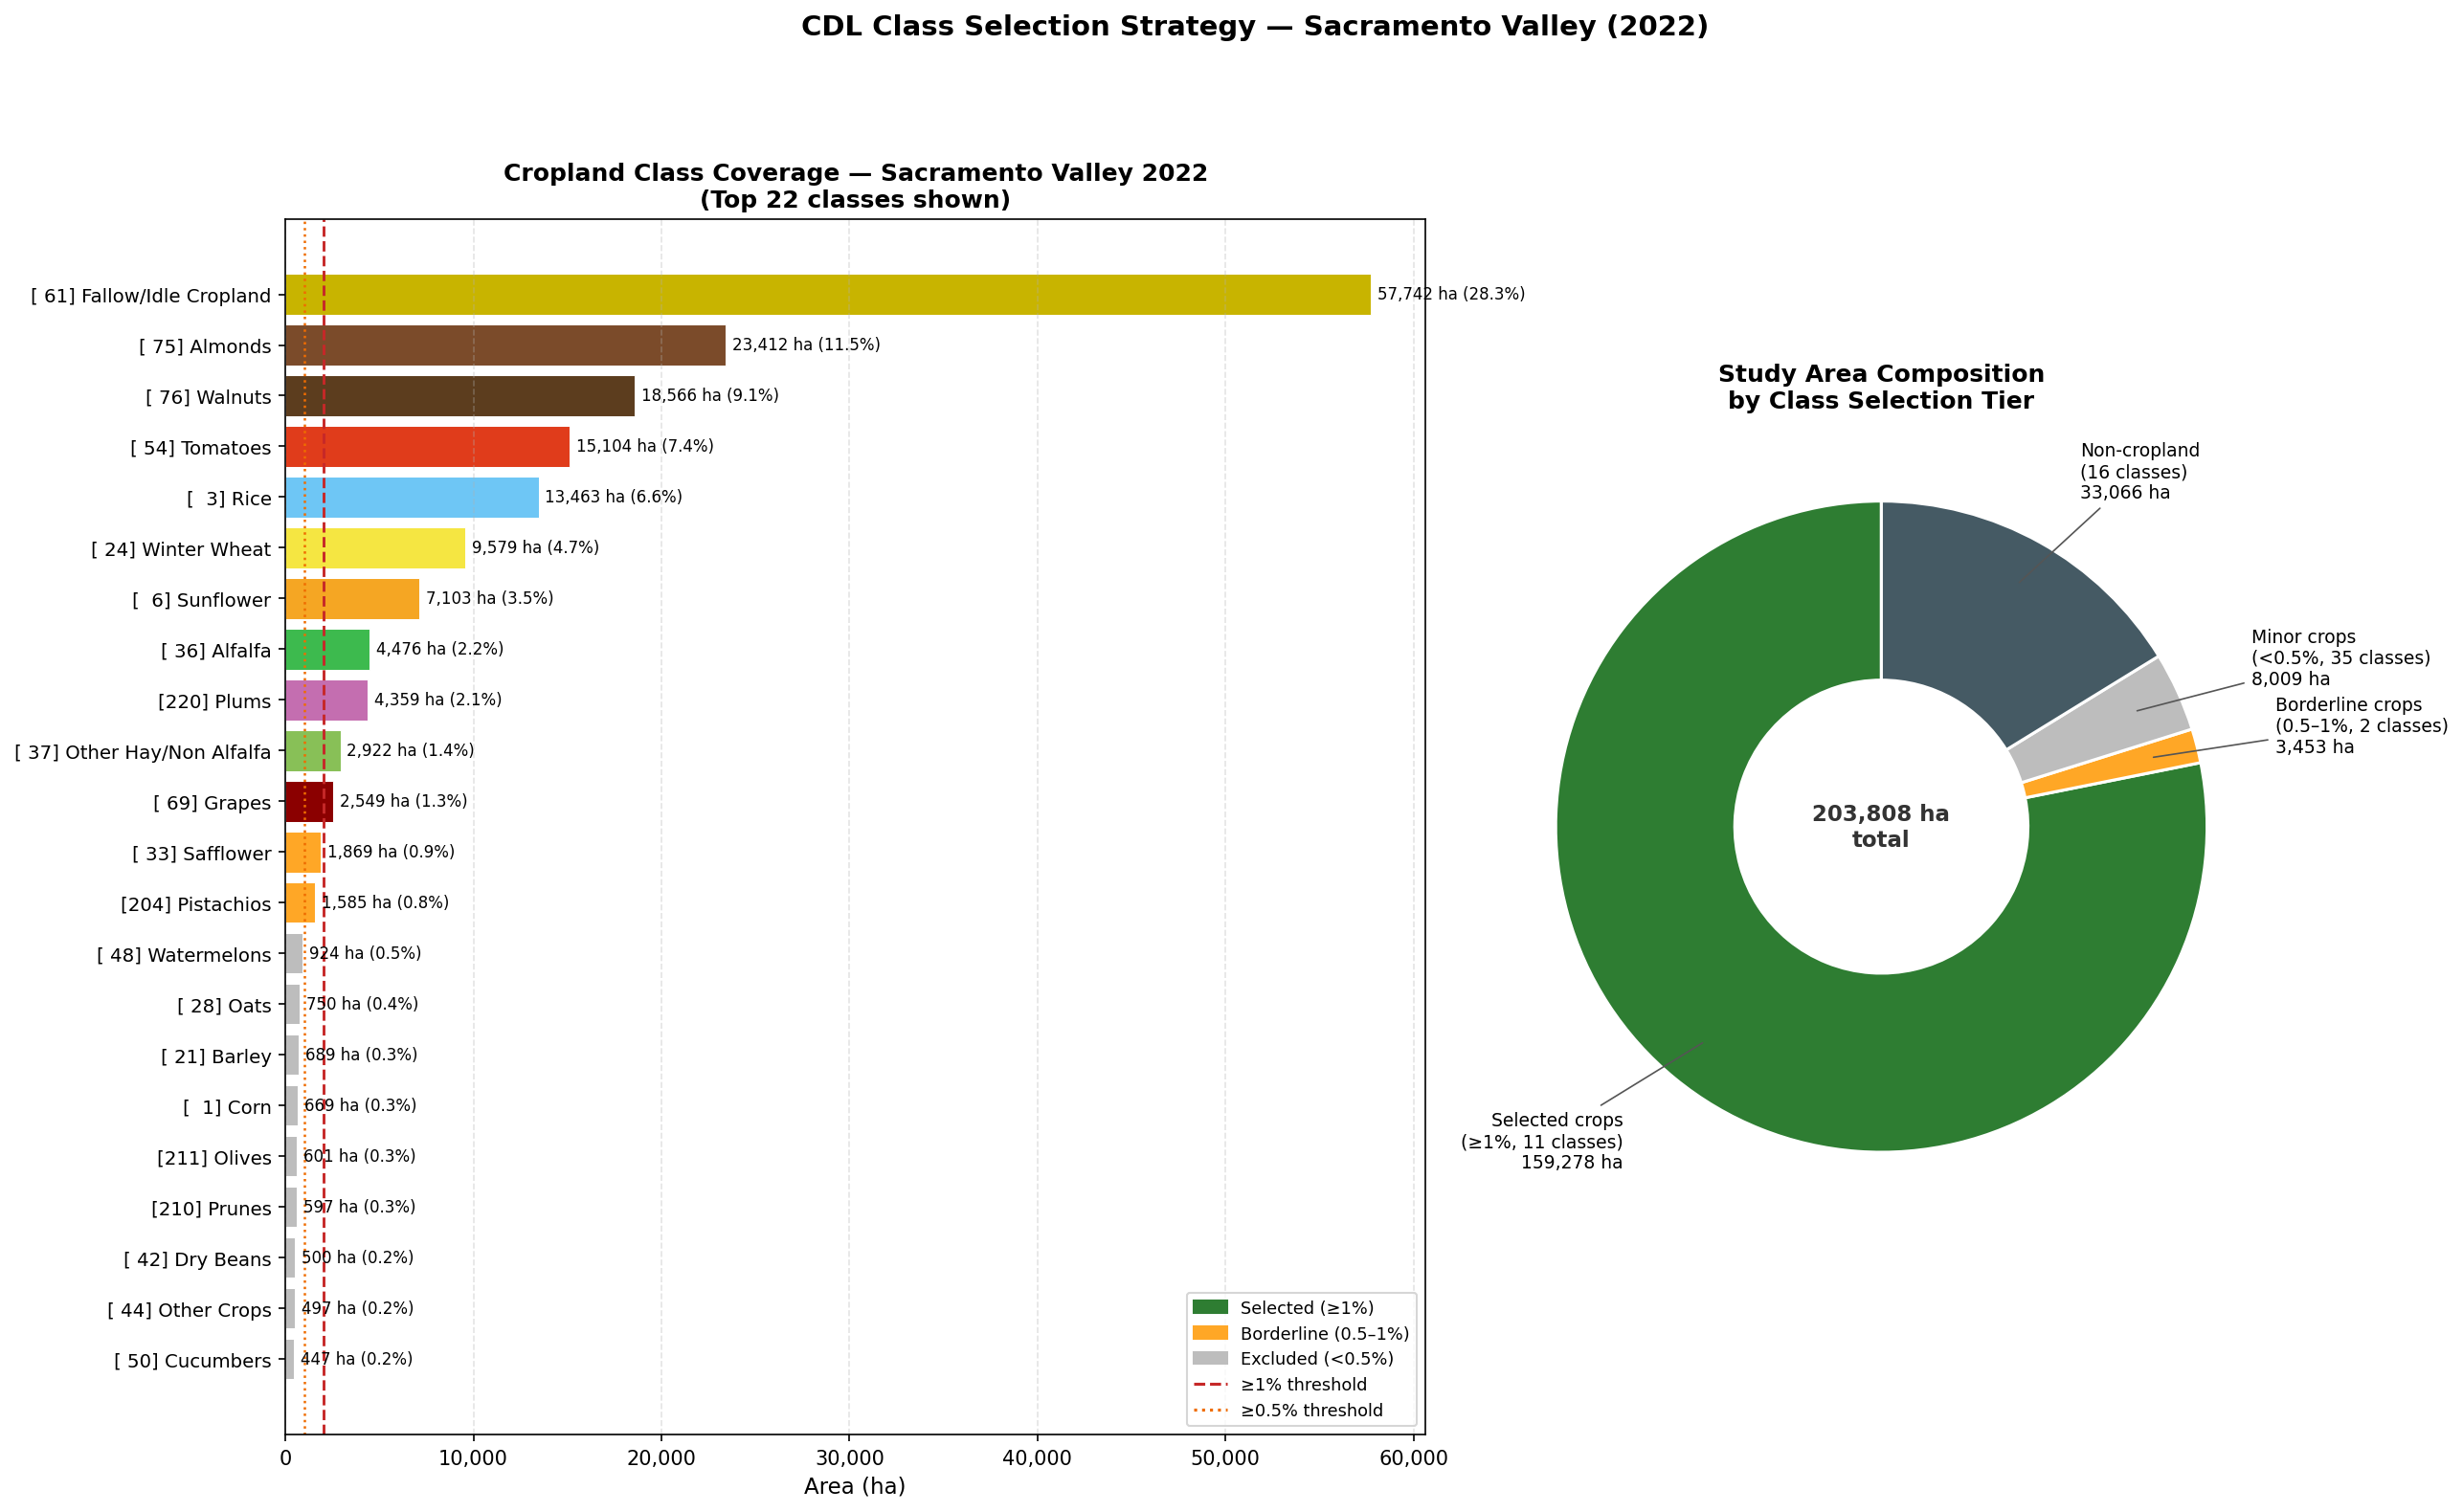
\includegraphics[width=\textwidth]{figures/cdl_class_selection_strategy.png}
    \caption{Distribusi kelas CDL dan strategi seleksi kelas untuk pelatihan model. Kelas dengan cakupan $\geq 1\%$ dipilih sebagai kelas target (hijau), kelas 0{,}5--1\% sebagai kandidat eksperimen lanjutan (oranye), dan kelas $<0{,}5\%$ dikecualikan (abu-abu).}
    \label{fig:cdl_class_selection}
\end{figure}

Tabel~\ref{tab:selected_classes} menampilkan 11 kelas yang terpilih beserta justifikasinya.

\begin{table}[htbp]
\centering
\caption{Kelas CDL Terpilih untuk Pelatihan Model ($\geq 1\%$ cakupan area studi)}
\label{tab:selected_classes}
\begin{tabular}{rlrrrr}
\hline
\textbf{No.} & \textbf{Kelas} & \textbf{ID} & \textbf{\% Tanaman} & \textbf{Area (ha)} & \textbf{Area (km$^2$)} \\
\hline
1  & Fallow/Idle Cropland  & 61  & 33,8\% & 57.742 & 577,42 \\
2  & Almonds               & 75  & 13,7\% & 23.412 & 234,12 \\
3  & Walnuts               & 76  & 10,9\% & 18.566 & 185,66 \\
4  & Tomatoes              & 54  &  8,8\% & 15.104 & 151,04 \\
5  & Rice                  & 3   &  7,9\% & 13.463 & 134,63 \\
6  & Winter Wheat          & 24  &  5,6\% &  9.579 &  95,79 \\
7  & Sunflower             & 6   &  4,2\% &  7.103 &  71,03 \\
8  & Alfalfa               & 36  &  2,6\% &  4.476 &  44,76 \\
9  & Plums                 & 220 &  2,6\% &  4.359 &  43,59 \\
10 & Other Hay/Non Alfalfa & 37  &  1,7\% &  2.922 &  29,22 \\
11 & Grapes                & 69  &  1,5\% &  2.549 &  25,49 \\
-- & Background (lainnya)  & 0   &    --   &    --  &     -- \\
\hline
\multicolumn{3}{l}{\textbf{Total kelas terpilih}} & \textbf{93,3\%} & \textbf{159.278} & \textbf{1.592,8} \\
\hline
\end{tabular}
\end{table}

Terdapat tiga justifikasi ilmiah untuk ambang batas $\geq 1\%$ yang digunakan:

\begin{enumerate}
    \item \textbf{Kecukupan sampel untuk \textit{deep learning}.}
    Kelas dengan cakupan $\geq 1\%$ menempati $\geq 2.038$ ha di area studi.
    Pada ukuran patch $256 \times 256$ piksel dengan resolusi 10 m ($\approx 510$ ha/patch), cakupan tersebut menghasilkan representasi spasial yang memadai dari ratusan petak lahan pertanian yang berbeda, sehingga model dapat mempelajari fitur spektral dan spasial yang dapat digeneralisasi.
    Kelas di bawah 1\% ($<$2.000 ha) umumnya tampil sebagai fragmen poligon yang tersebar dan kecil, sehingga tidak menyediakan keragaman spasial yang cukup untuk pelatihan segmentasi berbasis CNN \citep{alamimachichi2023}.

    \item \textbf{Ketidakseimbangan kelas yang dapat ditangani.}
    Himpunan kelas terpilih menghasilkan rasio ketidakseimbangan maksimum sebesar 22{,}6:1 (Fallow 57.742 ha vs.\ Grapes 2.549 ha).
    Rasio ini masih dapat ditangani dengan teknik standar seperti \textit{inverse-frequency class weighting} atau \textit{Focal Loss} tanpa menyebabkan ketidakstabilan pelatihan.
    Memasukkan kelas di bawah 0{,}5\% akan mendorong rasio ini di atas 100:1, yang melampaui kemampuan koreksi teknik pembobotan standar \citep{luo2024}.

    \item \textbf{Relevansi pertanian Sacramento Valley.}
    Kesebelas kelas yang terpilih merepresentasikan komoditas pertanian dominan Sacramento Valley berdasarkan statistik produksi tahunan USDA NASS \citep{copenhaver2021}:
    \textit{Almonds} dan \textit{Walnuts} merupakan tanaman pohon utama California yang bersama-sama mencakup 420 km$^2$;
    \textit{Tomatoes} mencerminkan posisi Sacramento Valley sebagai pusat produksi tomat olahan;
    \textit{Rice} memiliki tanda spektral yang khas akibat periode penggenangan sawah;
    dan \textit{Fallow/Idle Cropland} penting untuk pemantauan rotasi tanaman dan intensitas pertanian \citep{maleki2024}.
\end{enumerate}

Dua kelas tambahan, yaitu \textit{Safflower} (ID 33, 0{,}92\%) dan \textit{Pistachios} (ID 204, 0{,}78\%), berada di batas ambang dan akan dievaluasi dalam eksperimen lanjutan dengan 13 kelas untuk menilai apakah fenologi khasnya dapat mengompensasi jumlah sampel yang lebih kecil.

\subsection{Histogram per Band dan Korelasi}
Distribusi nilai reflectance dari band B2, B3, dan B4 terkonsentrasi di bawah 2000. 
Band \textit{red edge} (B5, B6, B7) memiliki distribusi lebih besar. 
Band NIR (B8) menunjukkan reflectance tinggi dengan distribusi yang lebih merata.
Korelasi antar band cahaya tampak (B2, B3, B4) sangat tinggi ($\ge 0,94$).

\subsection{Perubahan Indeks Vegetasi}
NDVI meningkat pada bulan April dan Juli yang menandakan awal musim tanam, lalu turun kembali menjelang akhir tahun yang mengindikasikan masa panen.

\section{Data Preprocessing}
Tahap preprocessing data bertujuan untuk memastikan citra satelit dan data label tutupan lahan memiliki kualitas spasial dan spektral yang konsisten.

\subsection{Cloud Masking dan Shadow Masking}
Tahap awal adalah \textit{cloud masking} dan \textit{shadow masking} pada citra Sentinel-2 menggunakan fungsi bawaan GEE berdasarkan persentase tutupan awan (CLOUDY\_PIXEL\_PERCENTAGE) yang rendah ($\le 10\%$).

\subsection{Citra Komposit Temporal}
Citra dikompositkan secara temporal menggunakan fungsi \textit{median reducer} untuk menghasilkan satu citra per interval 15 hari.

\subsection{Resampling Citra}
Dilakukan proses \textit{resampling} spasial menggunakan metode \textit{nearest neighbour} untuk menyamakan resolusi dan sistem proyeksi antara citra Sentinel-2 (10m) dan data label CDL (30m).

\subsection{Histogram Matching}
Metode \textit{histogram matching} diterapkan pada masing-masing band citra Sentinel-2 untuk menyamakan kontras warna piksel dengan label sama \citep{wang2023}.

\subsection{Patching dan Normalisasi Citra}
Citra dan data label dipotong menjadi patch berukuran $256\times256$ piksel. 
Setiap patch dinormalisasi menggunakan \textit{min-max normalization} ke rentang 0 hingga 1:
\begin{equation}
    x_{norm} = \frac{x - x_{min}}{x_{max} - x_{min}}
\end{equation}

\subsection{Seleksi Band Spektral--Temporal}

Penelitian ini mengusulkan metode seleksi fitur tiga tahap (\textit{3-stage feature selection}) yang dirancang khusus untuk citra Sentinel-2 multi-temporal pada tugas \textit{semantic segmentation}. Tujuannya adalah mengurangi redundansi spektral dan temporal tanpa mengorbankan performa segmentasi, sekaligus menekan biaya komputasi pelatihan model.

\subsubsection{Tahap 1 — Filter Preselection}

Tahap pertama bertujuan mereduksi seluruh channel masukan menjadi sekitar 25 kandidat terbaik menggunakan dua ukuran statistik yang murah secara komputasi.

\textbf{Global Separation Index (GSI).}
Untuk setiap band $b$, dihitung nilai separabilitas antar kelas:
\begin{equation}
    SI_{s,o}^{(b)} = \frac{|\mu_s^{(b)} - \mu_o^{(b)}|}{1{,}96 \times (\sigma_s^{(b)} + \sigma_o^{(b)})}
\end{equation}
di mana $\mu_s$, $\sigma_s$ adalah rata-rata dan standar deviasi kelas $s$, dan $\mu_o$, $\sigma_o$ untuk kelas pembanding $o$. Nilai GSI merupakan rata-rata $SI_{s,o}$ atas seluruh pasangan kelas.

\textbf{RF Feature Importance.}
Nilai kepentingan fitur diperoleh dari Random Forest yang dilatih pada sampel piksel berlabel:
\begin{equation}
    \text{RF}_{b} = \frac{\Delta \text{impurity}_b}{\sum_{b'} \Delta \text{impurity}_{b'}}
\end{equation}

\textbf{Joint Score.}
Kedua skor dinormalisasi ke rentang $[0,1]$ lalu digabungkan:
\begin{equation}
    \text{Score}_b = \alpha \cdot \text{GSI}_{\text{norm},b} + (1 - \alpha) \cdot \text{RF}_{\text{norm},b}
\end{equation}
dengan $\alpha = 0{,}5$ (bobot seimbang). Band dengan skor $\text{Score}_b$ tertinggi dipilih sebagai kandidat Tahap 2.

\subsubsection{Tahap 2 — CNN Forward Selection}

Tahap kedua menggunakan model segmentasi ringan (U-Net dengan encoder ResNet-18) sebagai \textit{oracle} seleksi. Algoritma \textit{sequential forward selection} secara greedy menambahkan band satu per satu berdasarkan urutan \textit{joint score} dari Tahap 1, dan mempertahankan band tersebut hanya apabila mIoU validasi meningkat melebihi ambang batas $\delta$:

\begin{equation}
    \text{terima band } b \iff \text{mIoU}_{t+1} > \text{mIoU}_{t} + \delta
\end{equation}

dengan $\delta = 0{,}005$. Proses dihentikan apabila tidak terjadi peningkatan selama tiga penambahan berturut-turut, atau jumlah band mencapai batas maksimum. Setiap iterasi melatih model selama 15 epoch dengan \textit{early stopping} (patience = 5) untuk efisiensi komputasi.

Metode ini merupakan kontribusi baru yang membedakan penelitian ini dari pendekatan sebelumnya. Pada studi terdahulu \citep{li2023hetao}, seleksi band dilakukan menggunakan GSI dan eliminasi fitur berbasis Random Forest sebagai \textit{filter} statis, di mana model segmentasi hanya digunakan setelah proses seleksi selesai. Dalam penelitian ini, model segmentasi sendiri bertindak sebagai \textit{oracle} dalam loop seleksi, sehingga kriteria pemilihan fitur sepenuhnya dioptimalkan terhadap metrik segmentasi (mIoU) daripada metrik klasifikasi piksel.

\subsubsection{Tahap 3 — Validasi Model Penuh}

Tiga himpunan band dilatih menggunakan tiga arsitektur segmentasi penuh untuk mengevaluasi dampak seleksi:

\begin{enumerate}
    \item \textbf{Eksperimen A} — semua band (baseline)
    \item \textbf{Eksperimen B} — band pilihan Tahap 1 (filter saja)
    \item \textbf{Eksperimen C} — band pilihan Tahap 2 (CNN forward selection)
\end{enumerate}

Setiap eksperimen dilatih dengan U-Net, DeepLabV3+, dan SegFormer selama 100 epoch. Metrik yang dibandingkan meliputi mIoU, IoU per kelas, F1-score, waktu pelatihan per epoch, dan penggunaan memori GPU.

\subsection{Label Filtering}
Berdasarkan seleksi kelas yang dijelaskan pada Subbagian~\ref{subsec:class_selection}, diterapkan proses \textit{label filtering} pada data CDL.
Sebelas kelas tanaman dengan cakupan $\geq 1\%$ (ID: 3, 6, 24, 36, 37, 54, 61, 69, 75, 76, 220) dipertahankan sebagai kelas target, sedangkan seluruh kelas lainnya---termasuk perairan, permukiman, lahan basah, dan kelas tanaman minor---diubah menjadi kelas \textit{background} (nilai 0).

\section{Pelatihan Model}
\subsection{Penerapan Attention Mechanism}
Pelatihan model \textit{semantic segmentation} menggunakan DeepLabV3+ dan SegFormer.
Untuk DeepLabV3+, ditambahkan \textit{Convolutional Block Attention Module} (CBAM) setelah ASPP \citep{hsu2022}.
SegFormer menggunakan \textit{Self-Attention} bawaan \citep{xie2021}.

\subsection{Skenario Pelatihan}
Skenario pelatihan meliputi:
\begin{enumerate}
    \item \textbf{Single Band Single date}: Setiap band dilatih terpisah pada tanggal tertentu.
    \item \textbf{Kombinasi Band Spektral Multi-temporal}: Menggunakan kombinasi GSI tertinggi dan data temporal.
\end{enumerate}

\subsection{Hyperparameter Tuning}
Dilakukan penyesuaian \textit{learning rate}, \textit{batch size}, dan \textit{epoch}.

\section{Evaluasi}
Metrik evaluasi yang digunakan:
\begin{itemize}
    \item \textbf{Overall Accuracy (OA)}: Mengukur proporsi piksel yang benar \citep{thomasramos2024}.
    \item \textbf{Mean Intersection over Union (mIoU)}: Rata-rata IoU seluruh kelas.
    \item \textbf{F1-score}: Rata-rata harmonik precision dan recall.
\end{itemize}
Dilakukan juga \textit{error analysis} dan pengukuran \textit{inference time}.


\chapter{HASIL DAN PEMBAHASAN}
\section{Hasil Eksperimen}
\textit{[Bagian ini akan berisi hasil eksperimen dari pemetaan tanaman pertanian menggunakan model semantic segmentation. Tabel dan grafik hasil akurasi (OA, mIoU, F1-score) akan ditampilkan di sini.]}

\section{Analisis Hasil}
\textit{[Bagian ini akan membahas analisis dari hasil yang didapatkan. Perbandingan antar model (DeepLabV3+ vs SegFormer), pengaruh kombinasi band, dan analisis kesalahan (error analysis) akan dijabarkan secara mendetail.]}

\subsection{Perbandingan Performa Model}
\textit{[Diskusi mengenai model mana yang lebih unggul dalam berbagai skenario]}

\subsection{Pengaruh Data Multi-Temporal}
\textit{[Diskusi mengenai apakah data multi-temporal meningkatkan akurasi dibandingkan single-date]}

\subsection{Analisis Kesalahan}
\textit{[Visualisasi dan pembahasan mengenai area yang sering salah diklasifikasikan]}


\chapter{KESIMPULAN DAN SARAN}
% ============================================================
% BAB KESIMPULAN DAN SARAN
% ============================================================
% NOTE (2026-03-04): Kesimpulan ini ditulis berdasarkan hasil
% eksperimen skala kecil (3 tanggal Januari 2022, 15 epoch).
% Bagian yang ditandai [*] perlu diperbarui setelah eksperimen
% skala penuh dengan 72 tanggal selesai.
% ============================================================

\section{Kesimpulan}

Berdasarkan hasil eksperimen dan analisis yang telah dilakukan, penelitian ini menghasilkan
kesimpulan sebagai berikut yang menjawab tiga rumusan masalah penelitian:

\begin{enumerate}

    \item \textbf{Perbandingan akurasi \textit{single-date} versus \textit{multi-temporal}.}

    Pada eksperimen skala kecil dengan tiga tanggal akuisisi Januari 2022 dan 10 kelas
    tanaman aktif (tanpa \textit{Fallow/Idle}), pendekatan \textit{multi-temporal} naif
    (Exp B, 27 channel, mIoU SegFormer = 0.2519) tidak menunjukkan keunggulan yang
    signifikan dibandingkan pendekatan \textit{single-date}
    (Exp A, 9 channel, mIoU SegFormer = 0.2556).
    Hasil ini disebabkan oleh keterbatasan variasi temporal --- ketiga tanggal yang tersedia
    semuanya berasal dari bulan Januari sehingga tidak merepresentasikan siklus fenologi
    lengkap.
    Bukti manfaat multi-temporal paling terlihat pada kelas \textit{Winter Wheat}, yang
    mengalami peningkatan IoU terbesar dari Exp A ke Exp B (27.13\% $\rightarrow$ 35.52\%
    pada SegFormer), mengonfirmasi bahwa informasi temporal yang relevan membantu
    membedakan tanaman dengan karakteristik fenologi musim yang berbeda.
    Eksperimen skala penuh dengan 72 tanggal yang mencakup seluruh siklus tanam
    diharapkan menunjukkan keunggulan multi-temporal yang lebih nyata.~[*]

    \item \textbf{Efektivitas \textit{pipeline} seleksi band tiga tahap.}

    \textit{Pipeline} seleksi band yang diusulkan --- terdiri dari \textit{Global Separation
    Index} (GSI), \textit{Random Forest feature importance}, dan \textit{CNN forward
    selection} berbasis mIoU --- berhasil mengidentifikasi subset band optimal sebanyak
    $K^* = 4$ band dari total fitur yang tersedia.
    Band yang terpilih adalah B11 (1 Jan), B12 (1 Jan), B12 (31 Jan), dan B8A (1 Jan),
    yang merepresentasikan region SWIR dan \textit{Red Edge} --- dua kawasan spektral
    paling diskriminatif untuk vegetasi pertanian.
    Dengan hanya 4 channel (efisiensi 85.2\% dari 27 channel Exp B), Exp C mempertahankan
    akurasi yang sebanding: penurunan mIoU hanya 1.98 poin pada SegFormer
    (0.2519 $\rightarrow$ 0.2321).
    Hasil ini memvalidasi hipotesis kedua bahwa subset band hasil seleksi dapat
    mempertahankan akurasi segmentasi yang kompetitif dengan beban komputasi yang
    jauh lebih rendah.

    \item \textbf{Perbandingan kinerja DeepLabV3+CBAM dan SegFormer.}

    SegFormer (encoder MiT-B2) secara konsisten mengungguli DeepLabV3+CBAM (encoder
    ResNet-50 dengan CBAM) pada seluruh konfigurasi input.
    Selisih mIoU berkisar antara 1.49 hingga 2.83 poin: Exp A (+2.83 poin),
    Exp B (+1.49 poin), dan Exp C (+1.66 poin).
    Keunggulan ini konsisten dengan hipotesis ketiga bahwa mekanisme
    \textit{Efficient Self-Attention} pada SegFormer lebih efektif menangkap konteks
    spasial global yang relevan untuk membedakan petak-petak lahan pertanian berskala
    besar dalam citra Sentinel-2.
    Sebaliknya, keunggulan konvolusi lokal DeepLabV3+CBAM relatif lebih terbatas pada
    data resolusi 10 meter yang memiliki batas antar kelas yang gradual.

\end{enumerate}

Secara keseluruhan, penelitian ini membuktikan bahwa \textit{pipeline} tiga tahap yang
mengintegrasikan seleksi fitur spektral-temporal dengan model \textit{semantic segmentation}
adalah pendekatan yang layak untuk pemetaan tanaman berbasis citra Sentinel-2.
SegFormer dengan input 4 channel hasil seleksi terbukti mampu menghasilkan akurasi
yang mendekati konfigurasi penuh dengan efisiensi komputasi yang lebih tinggi.

\section{Saran}

Berdasarkan temuan dan keterbatasan penelitian ini, berikut adalah saran untuk
pengembangan penelitian selanjutnya:

\begin{enumerate}

    \item \textbf{Eksperimen skala penuh dengan data 72 tanggal.}
    Eksperimen skala kecil ini perlu diulang menggunakan seluruh dataset multi-temporal
    (72 tanggal, 2022--2024) agar pengaruh informasi fenologi sepanjang siklus musim
    tanam dapat terukur secara definitif.
    Hasil eksperimen skala penuh akan menjadi dasar kesimpulan akhir yang lebih valid
    mengenai keunggulan pendekatan \textit{multi-temporal}.

    \item \textbf{Penanganan ketidakseimbangan kelas.}
    Kelas minoritas seperti \textit{Other Hay} (IoU 3--4\%) dan \textit{Alfalfa}
    (IoU 8--18\%) secara konsisten menunjukkan performa rendah akibat distribusi kelas
    yang tidak seimbang.
    Penelitian selanjutnya disarankan mengeksplorasi strategi seperti \textit{class-weighted
    loss}, \textit{focal loss}, atau oversampling patch berbasis kelas minoritas untuk
    meningkatkan akurasi pada kelas yang langka.

    \item \textbf{Pengujian generalisasi antar area studi.}
    Penelitian ini dibatasi pada Sacramento Valley, California.
    Untuk mengevaluasi kemampuan generalisasi model dan \textit{pipeline} seleksi band,
    perlu dilakukan pengujian pada area studi lain --- misalnya San Joaquin Valley
    (California) atau kawasan pertanian di luar Amerika Serikat --- dengan pola tanam
    dan jenis tanaman yang berbeda.

    \item \textbf{Pengembangan \textit{pipeline} seleksi band.}
    \textit{Pipeline} seleksi band yang diusulkan menggunakan U-Net ResNet-18 sebagai
    \textit{oracle} pada Stage 2 untuk efisiensi komputasi.
    Penelitian selanjutnya dapat membandingkan oracle ini dengan model alternatif
    (misalnya SegFormer-B0) atau mengganti \textit{sequential forward selection} dengan
    metode yang lebih efisien secara komputasi seperti \textit{mutual information}-based
    selection atau \textit{LASSO regularization} agar seleksi dapat dilakukan pada ruang
    fitur yang lebih besar.

    \item \textbf{Integrasi \textit{encoder} temporal eksplisit.}
    Pendekatan \textit{multi-temporal} pada penelitian ini menggunakan penggabungan
    band secara naif (\textit{channel stacking}).
    Penggunaan modul temporal eksplisit --- seperti \textit{Long Short-Term Memory} (LSTM),
    \textit{Temporal Self-Attention}, atau \textit{TimeSformer} --- yang secara arsitektural
    memisahkan dimensi temporal dan spasial diharapkan dapat mengekstraksi pola fenologi
    lebih efektif dibandingkan \textit{channel stacking}.

\end{enumerate}


\bibliographystyle{apalike}
\bibliography{references}

\end{document}
